% !TEX root = IBL-InsolvabilityOfQuintic.tex
\chapter{Algebraic extension fields}
\label{chapter:AlgebraicExtensions}
\thispagestyle{empty}


Our goal remains: to show that there exist polynomials that are \emph{not} solvable by radicals over $\mathbb{Q}$. In Chapter~\ref{chapter:SolvabilityByRadicals}, we finally succeeded in properly formulating the notion of solvability by radicals, which we did in the language of field extensions. Additionally, we were able to catalog many polynomials that we are certain are solvable by radicals. Then, in Chapter~\ref{chapter:Rings}, we took a much closer look a polynomials, ultimately building a significant amount of language and theory to analyze polynomial rings over fields. The conclusion of the chapter hinted at the tight connection between polynomial rings and field extensions where we saw that $\mathbb{Q}[x]/(x^2+1) \cong \mathbb{Q}(i)$. In this chapter, we will clarify this connection and exploit it to significantly deepen our understanding of extension fields of the form $\mathbb{Q}(\alpha)$ where $\alpha$ is a root of some polynomial in $\mathbb{Q}[x]$. 


% % % % % % % % % % % % % % % % % % % % % % % % % % % % % % % % % % % % % % % % % % % %
% % % % % % % % % % % % % % % % % % % % % % % % % % % % % % % % % % % % % % % % % % % %
% SECTION
% % % % % % % % % % % % % % % % % % % % % % % % % % % % % % % % % % % % % % % % % % % %
% % % % % % % % % % % % % % % % % % % % % % % % % % % % % % % % % % % % % % % % % % % %
\section{Algebraic elements}

Recall that a polynomial in $F[x]$ is solvable by radicals over $F$ if all of the roots of the polynomial lie in some radical extension of $F$. Our focus is on roots of polynomials, and the next definition gives us some language to highlight this.

\begin{definition}
Let $F$ be a subfield of $E$. An element $\alpha\in E$ is \textbf{algebraic} over $F$ if $p(\alpha) = 0$ for some nonzero $p(x)\in F[x]$. If $\alpha$ is not algebraic over  $F$, then it is said to be \textbf{transendental} over $F$. 
\end{definition}

To show an element $\alpha$ is algebraic over $F$, we need only produce a polynomial \emph{with coefficients in $F$} for which $\alpha$ is a root. For example, the complex number $\sqrt{2}$ is algebraic over $\mathbb{Q}$ because $\sqrt{2}$ is a root of $p(x) = x^2 - 2$ and $p(x) \in \mathbb{Q}[x]$. Also, $\pi$ is algebraic over $\mathbb{R}$ because $\pi$ is a root of $q(x) = x-\pi$ and $q(x) \in \mathbb{R}[x]$. However, it is \emph{much} harder to show that $\pi$ is \emph{not} algebraic over $\mathbb{Q}$ (so  $\pi$ is transcendental over $\mathbb{Q}$). Incidentally, a set-theoretic argument  shows that almost all elements of $\mathbb{C}$ are transcendental over $\mathbb{Q}$; nevertheless, we will focus on algebraic elements.

\begin{problem}
Show that each of the following are algebraic over $\mathbb{Q}$: $11$, $\sqrt[3]{11}$, $\zeta_{11}$, and $i$.
\end{problem}

\begin{problem}
Suppose that $\gamma \in \mathbb{C}$ and $\gamma^5 = 2\gamma^2 -7$. Explain why $\gamma$ is algebraic over $\mathbb{Q}$.
\end{problem}

\begin{problem}\label{prob.Sqrt2PlusIIsAlgebraic}
Let $\alpha = \sqrt{2} + i$. Show that $\alpha$ is algebraic over $\mathbb{Q}$.
\end{problem}

Now, an algebraic element over $F$ is a root of \emph{some} nonzero polynomial over $F$, but such an element will be a root of lots of polynomials. For example, since $\sqrt{2}$ is a root of $p(x) = x^2 - 2$, we find that for \emph{every} $q(x)\in \mathbb{Q}[x]$, $\sqrt{2}$ is a root of $q(x)p(x)$ because $q(\sqrt{2})p(\sqrt{2}) =  q(\sqrt{2})p(0) =0$. The polynomial $x^2 - 2$ is special because it is a polynomial \emph{of smallest degree} for which $\sqrt{2}$ is a root. In order to formalize this observation, we need to weave together several results from the last chapter. 

Let $F$ be a subfield of $E$, and suppose that $\alpha\in E$ is algebraic over $F$. Then $\alpha$ is the root of \emph{some} nonzero $p(x)\in F[x]$.  Let's look at the set of \emph{all} polynomials for which $\alpha$ is a root: $I = \{p(x)\in F[x]\mid p(\alpha) = 0\}$. By Theorem~\ref{thm.EvalHom}, ``evaluation at $\alpha$'' gives rise to a homomorphism $\mathcal{E}_\alpha: F[x] \to E[x]$, and notice that $I$ is precisely the kernel of $\mathcal{E}_\alpha$. Thus, by Theorem~\ref{thm.KernelIsIdealImageIsSubring}, $I$ is an ideal of $F[x]$, and since $F[x]$ is a PID, it must be that $I = (m(x))$ for some $m(x) \in F[x]$. 

Now, $m(x)$ is nonzero since $I$ contains some nonzero polynomial, and this also implies that $m(x)$ is not a constant polynomial since the only constant polynomial that has roots is the zero polynomial. Moreover, if $m(x)$ is not monic, we can make it monic by multiplying by the inverse of the leading coefficient and the result will still generate $I$ by Theorem~\ref{thm.DifferByUnitSameIdeal}. So, we may assume that $I = (m(x))$ with $m(x)$ nonconstant and monic. 

Also, notice that by Theorem~\ref{thm.PrincipalIdeals}, $m(x)$ divides every polynomial in $I$. So if $I = (n(x))$ for some other monic polynomial $n(x)$, then $m(x)$ and $n(x)$ would divide each other. In other words, $m(x) = a(x)n(x) = a(x)b(x)m(x)$ for some polynomials $a(x),b(x)\in F[x]$. Considering the degree of both sides of $m(x) = a(x)b(x)m(x)$, we see that $a(x)$ and $b(x)$ must be constant polynomials. But since $m(x) = a(x)n(x)$ with $m(x)$ and $n(x)$ both monic, the only conclusion is that $a(x) = 1$, so $m(x) = n(x)$. 

In summary, $I= \{p(x)\in F[x]\mid p(\alpha) = 0\}$ is an ideal, and there is a unique nonconstant monic polynomial $m(x)$ that generates $I$. In fact, more is true. 

\begin{lemma}\label{lem.MinimalPolyIsIrreducible}
Let $F$ be a subfield of $E$, and suppose that $\alpha\in E$ is algebraic over $F$. Let $I = \{p(x)\in F[x]\mid p(\alpha) = 0\}$, and suppose that $I = (m(x))$ for some nonconstant $m(x) \in F[x]$. Then $m(x)$ is irreducible.
\end{lemma}

Combining Lemma~\ref{lem.MinimalPolyIsIrreducible} with our previous discussion, we arrive at the following fact.

\begin{fact}\label{fact.ExistsMinimalPoly}
Let $F$ be a subfield of $E$, and suppose that $\alpha\in E$ is algebraic over $F$. Then there is a unique irreducible monic polynomial $m(x) \in F[x]$ such that $m(\alpha) = 0$. Moreover, if $p(x) \in F[x]$ and $p(\alpha) = 0$, then $m(x)$ divides $p(x)$.
\end{fact}

The polynomial $m(x)$ from  Fact~\ref{fact.ExistsMinimalPoly} gets a special name.

\begin{definition}
Suppose that $\alpha\in E$ is algebraic over $F$. The unique irreducible monic polynomial $m(x) \in F[x]$ such that $m(\alpha) = 0$ is called the \textbf{minimal polynomial} of $\alpha$ over $F$. The \textbf{degree} of $\alpha$ over $F$ is defined to be the degree of the minimal polynomial of $\alpha$ over $F$. 
\end{definition}

\begin{theorem}
Let $F$ be a subfield of $E$. Suppose that $\alpha\in E$ is algebraic over $F$, and let $m(x)$ be the minimal polynomial of $\alpha$ over $F$. If $V = \{p(x)\in F[x]\mid p(\alpha) = 0\}$ (i.e~the set of all polynomials that vanish at $\alpha$), then $V = (m(x))$.
\end{theorem}


We will see shortly that the minimal polynomial of $\alpha$ over $F$ is key to understanding the field extension $F(\alpha)$. But how do we find the minimal polynomial of $\alpha$ over $F$? The first step is to find \emph{any} monic polynomial $p(x)\in F[x]$ for which $p(\alpha) = 0$ (which also verifies that $\alpha$ is algebraic over $F$). If we can show that $p(x)$ is irreducible, then $p(x)$ is the minimal polynomial, and we're done. Otherwise, we factor $p(x)$ into irreducible polynomials in $F[x]$, and  by Fact~\ref{fact.ExistsMinimalPoly}, the minimal polynomial will be whichever one of the factors has $\alpha$ as a root. Let's test this out with some examples. 

\begin{problem}\label{prob.MinPolyZeta3}
Explain why the minimal polynomial for $\zeta_3$ over $\mathbb{Q}$ is \textit{not} $x^3-1$. Find the minimal polynomial  $\zeta_3$ over $\mathbb{Q}$, and determine the degree of  $\zeta_3$ over $\mathbb{Q}$?
\end{problem}

\begin{problem}\label{prob.MinPolyCubeRoot11}
The polynomial $p(x) = x^3-11$ has three roots in $\mathbb{C}$. 
\begin{enumerate}
\item Find the degree over $\mathbb{Q}$ of each of the three roots.
\item Find the degree over $\mathbb{R}$ of each of the three roots.
\end{enumerate}
\end{problem}


\begin{problem}
The polynomial $p(x) = x^5-2x^3-3x$ has five roots in $\mathbb{C}$. Find the minimal polynomial over $\mathbb{Q}$ of each of the five roots.
\end{problem}

\begin{problem}
Let $z = a+bi$ with $a,b\in \mathbb{Q}$, and define $p(x) = (x-z)(x-\overline{z})$. Prove that $p(x)\in \mathbb{Q}[x]$, and then use this to find the minimal polynomial of $2+i$ over $\mathbb{Q}$.
\end{problem}

\begin{problem}
Find the minimal polynomial of $3-\sqrt{5}$ over $\mathbb{Q}$.
\end{problem}

% % % % % % % % % % % % % % % % % % % % % % % % % % % % % % % % % % % % % % % % % % % %
% SUBSECTION
% % % % % % % % % % % % % % % % % % % % % % % % % % % % % % % % % % % % % % % % % % % %
\subsection{Describing elements of $F(\alpha)$}

In Chapter~\ref{chapter:Fields}, we explored extension fields of the form $F(\alpha)$ where $\alpha$ was chosen from some larger field $E$. However, the definition of $F(\alpha)$ was abstract and often hard to work with. For example, $\mathbb{Q}(i)$ is defined to be the smallest subfield of $\mathbb{C}$ containing $\mathbb{Q}$ and $i$, but this doesn't tell us much about what the elements of $\mathbb{Q}(i)$ actually look like. Nevertheless, in Problem~\ref{prob.QAdjoinI}, we were able show that $\mathbb{Q}(i)$ is precisely the set of elements of the form $a+bi$ with $a,b\in \mathbb{Q}$, and we also succeeded in showing that $\mathbb{Q}(\sqrt{5}) = \{a+b\sqrt{5}\mid a,b\in \mathbb{Q}\}$. 

However, we noticed that describing $\mathbb{Q}(\alpha)$ is not always so easy since, for example, if $\alpha = \sqrt{2} + i$, then $\mathbb{Q}(\alpha) \neq \{a+b\alpha\mid a,b\in \mathbb{Q}\}$. That said, we've learned a lot since Chapter~\ref{chapter:Fields}, so let's take another go at trying to describe fields like $\mathbb{Q}(\alpha)$. 

Remember that (for $\alpha = \sqrt{2} + i$) we were able to show that $\{a+b\alpha\mid a,b\in \mathbb{Q}\} \subseteq \mathbb{Q}(\alpha)$, but the reverse containment did not hold. And, the reason the reverse containment didn't hold was because $\{a+b\alpha\mid a,b\in \mathbb{Q}\}$ is not a field, which can be seen fairly easily since $\alpha^2 \notin \{a+b\alpha\mid a,b\in \mathbb{Q}\}$ (so it's not closed under multiplication). 

So why not add in $\alpha^2$ and consider something like  $\{a+b\alpha + c\alpha^2\mid a,b,c\in \mathbb{Q}\}$? Remembering that $\mathbb{Q}(\alpha)$ is a field containg $\mathbb{Q}$ and $\alpha$ (and is closed under addition and multiplication), we see again that $\{a+b\alpha + c\alpha^2\mid a,b,c\in \mathbb{Q}\} \subseteq \mathbb{Q}(\alpha)$. So maybe $\{a+b\alpha + c\alpha^2\mid a,b,c\in \mathbb{Q}\} = \mathbb{Q}(\alpha)$. Or, maybe we need to look at $\{a+b\alpha + c\alpha^2 + d\alpha^3\mid a,b,c,d\in \mathbb{Q}\}$. These are all good ideas since $a_0+a_1\alpha + a_2\alpha^2 + a_3\alpha^3 + \cdots + a_n\alpha^n \in \mathbb{Q}(\alpha)$ whenever $a_0,a_1,a_2,a_3,\ldots,a_n\in \mathbb{Q}$. Let's formalize this.


\begin{theorem}
Let $F$ be a subfield of $E$, and let $\alpha\in E$. If $p(x)\in F[x]$, then $p(\alpha) \in F(\alpha)$.
\end{theorem}

\begin{problem}
Let $p(x) = 2x^3+7x^2-\frac{1}{2}$. We know that $\mathbb{Q}(\sqrt{5}) = \{a+b\sqrt{5}\mid a,b\in \mathbb{Q}\}$ by  Problem~\ref{prob.QAdjoinRoot5}. Verify directly that $p(\sqrt{5}) \in \mathbb{Q}(\sqrt{5})$ by writing $p(\sqrt{5})$ in the form $a+b\sqrt{5}$ for some $a,b\in \mathbb{Q}$.
\end{problem}

We are studying the elements we get when we plug $\alpha$ into polynomials. Let's frame this in terms of the evaluation homomorphism introduced in Theorem~\ref{thm.EvalHom}, like we did at the beginning of this chapter. The next theorem generalizes Problem~\ref{prob.EvalAtI}.

\begin{theorem}
Let $F$ be a subfield of $E$. Suppose that $\alpha\in E$ is algebraic over $F$, and let $m(x)$ be the minimal polynomial of $\alpha$ over $F$. If $\mathcal{E}_\alpha:F[x] \rightarrow E$ is the homomorphism defined by $\mathcal{E}_\alpha(p(x)) = p(\alpha)$, then 
\begin{enumerate}
\item $\ker\left(\mathcal{E}_\alpha\right)=(m(x))$, and
\item $\operatorname{im}\left(\mathcal{E}_\alpha\right)\subseteq F(\alpha)$ and $F\cup\{\alpha\}\subset \operatorname{im}\left(\mathcal{E}_\alpha\right)$.
\end{enumerate}
\end{theorem}

Using Theorems~\ref{thm.MaximalIFFIrreducibleinFx} and~\ref{thm.QuotientIsField} (and the First Isomorphism Theorem for Rings), we can deduce that the image of $\mathcal{E}_\alpha$ is a field. But then, if we can verify that the image of $\mathcal{E}_\alpha$ contains $F$ and $\alpha$, we can conclude that the image of $\mathcal{E}_\alpha$ is actually \emph{equal} to $F(\alpha)$ (by the definition of $F(\alpha)$). Let's put this together.

\begin{theorem}
Let $F$ be a subfield of $E$. Suppose that $\alpha\in E$ is algebraic over $F$, and let $m(x)$ be the minimal polynomial of $\alpha$ over $F$. Then 
$F(\alpha) \cong F[x]/(m(x)).$
\end{theorem}

Notice that we still haven't succeeded in providing a nice description $F(\alpha)$, but we will if we can find a nice description of $F[x]/(m(x))$.

\begin{lemma}\label{lem.DescribeQuotientWithRemainders}
Let $F$ be a subfield of $E$, and suppose that $\alpha\in E$ is algebraic over $F$. Let $m(x)$ be the minimal polynomial of $\alpha$ over $F$, and let $n$ be the degree of $\alpha$ over $F$.  If $a(x) + (m(x)) \in F[x]/(m(x))$, then $a(x) + (m(x)) =  r(x) + (m(x))$ where $r(x)$ is the remainder obtained when dividing $a(x)$ by $m(x)$. Consequently,
\[F[x]/(m(x)) = \{r(x) +  (m(x)) \mid \deg r(x) < n \text{ or } r(x) = 0\}.\]
\end{lemma}

Tying together all of our work, we finally arrive at our desired description of $F(\alpha)$.

\begin{theorem}\label{thm.DescribeFAdjoinr}
Let $F$ be a subfield of $E$. Suppose that $\alpha\in E$ is algebraic over $F$, and let $n$ be the degree of $\alpha$ over $F$. Then \[F(\alpha) = \{a_0 + a_1\alpha+\cdots+a_{n-1}\alpha^{n-1} \mid a_0,a_1,\ldots,a_{n-1} \in F\}.\]
\end{theorem}

We had to work hard for Theorem~\ref{thm.DescribeFAdjoinr}, but using it is fairly easy. For example, suppose we want to describe $\mathbb{Q}(\sqrt[3]{2})$. We first need to know the degree of $\sqrt[3]{2}$ over $\mathbb{Q}$. Of course, $\sqrt[3]{2}$ is a root of $m(x) = x^3-2$, and $m(x)$ is irreducible by Theorems~\ref{thm.nthRoots} and~\ref{thm.ReducibilityTestDegree2or3}. Thus, $m(x) = x^3-2$ is the minimal polynomial of $\sqrt[3]{2}$ over $\mathbb{Q}$, so $\sqrt[3]{2}$ has degree $3$ over $\mathbb{Q}$. Now we  apply Theorem~\ref{thm.DescribeFAdjoinr} to find that $\mathbb{Q}(\sqrt[3]{2}) = \{a_0 + a_1\sqrt[3]{2}+a_{2}(\sqrt[3]{2})^{2} \mid a_0,a_1,a_2 \in \mathbb{Q}\}$.

\begin{problem}
Use  Theorem~\ref{thm.DescribeFAdjoinr} to describe $\mathbb{Q}(\zeta_3)$.
\end{problem}

\begin{problem}\label{prob.Degree3ExtOfF3}
Let $p(x) = x^3-x+1 \in \mathbb{Z}_3[x]$, and let $r$ be a root of $p(x)$. 
\begin{enumerate}
\item Prove that $p(x)$ is irreducible in $\mathbb{Z}_3[x]$. 
\item Use Theorem~\ref{thm.DescribeFAdjoinr} to describe $\mathbb{Z}_3(r)$.
\item How many elements are in the field $\mathbb{Z}_3(r)$?
\end{enumerate}
\end{problem}

\begin{problem}\label{prob.DescribeQAdjoinSqrt2PlusI}
Let $\alpha = \sqrt{2} + i$. In Problem~\ref{prob.Sqrt2PlusIIsAlgebraic}, we saw that $\alpha$ is algebraic over $\mathbb{Q}$ since $\alpha$ is a root of  $x^4-2x^2+9\in \mathbb{Q}[x]$. Let $m(x)$ denote the minimal polynomial for $\alpha$ over $\mathbb{Q}$.
\begin{enumerate}
\item Use Theorem~\ref{thm.DescribeFAdjoinr} (and Problem~\ref{prob.QAdjoinI}) to explain why the degree of $m(x)$ isn't $1$ or $2$.
\item Use Fact~\ref{fact.ExistsMinimalPoly} to explain why $m(x)$ is a factor of $x^4-2x^2+9$.
\item Explain why the degree of $m(x)$ isn't $3$.
\item Explain why  $m(x)=x^4-2x^2+9$.
\item Use Theorem~\ref{thm.DescribeFAdjoinr} to describe $\mathbb{Q}(\sqrt{2} + i)$.
\end{enumerate}
\end{problem}

The next problem highlights how we use the minimal polynomial for $\alpha$ to compute (or rather, simplify) in  $F(\alpha)$.

\begin{problem}\label{prob.DescribeQRootx52x2}
The polynomial $p(x) = x^5 + 2x + 2$ is irreducible in $\mathbb{Q}[x]$ (you do not need to prove this). Let $s$ be a root of $p(x)$. By Theorem~\ref{thm.DescribeFAdjoinr}, every element of $\mathbb{Q}(s)$ can be written in the form $a_0 + a_1s + a_2s^2 + a_3s^3 + a_4s^4$ for some $a_0,a_1,a_2,a_3,a_4 \in \mathbb{Q}$.
\begin{enumerate}
\item Use the fact that $p(s) = 0$ to write $s^5$ in the form  $a_0 + a_1s + a_2s^2 + a_3s^3 + a_4s^4$.
\item Rewrite each of the following elements of $\mathbb{Q}(\alpha)$ in the form  $a_0 + a_1s + a_2s^2 + a_3s^3 + a_4s^4$.
\begin{enumerate}
\item $(s^3+2)(s^3+3s)$
\item $3s^4(2+s^3)(5-s+s^2)$
\end{enumerate}
\end{enumerate}
\end{problem}

\begin{problem}\label{prob.DescribeQAdjoinRoot2Andi}
Let's try to describe $\mathbb{Q}(\sqrt{2},i)$. Notice that $\mathbb{Q}(\sqrt{2},i) = \left(\mathbb{Q}(\sqrt{2})\right)(i)$. In words, the field obtained by adjoining $\sqrt{2} $ and $i$ at the same time is equal to the field obtained by first adjoining $\sqrt{2}$ and then adjoining $i$ to the result.
\begin{enumerate}
\item Use  Theorem~\ref{thm.DescribeFAdjoinr} to describe $\mathbb{Q}(\sqrt{2})$.
\item Use Theorem~\ref{thm.ReducibilityTestDegree2or3} to explain why $x^2+1$ is the minimal polynomial of $i$ over $\mathbb{Q}(\sqrt{2})$.
\item Use  Theorem~\ref{thm.DescribeFAdjoinr} to describe $\left(\mathbb{Q}(\sqrt{2})\right)(i)$, which is equal to $\mathbb{Q}(\sqrt{2},i)$.
\item How does your description of $\mathbb{Q}(\sqrt{2},i)$ compare to that for $\mathbb{Q}(\sqrt{2} + i)$ in Problem~\ref{prob.DescribeQAdjoinSqrt2PlusI}?
\end{enumerate}
\end{problem}


% % % % % % % % % % % % % % % % % % % % % % % % % % % % % % % % % % % % % % % % % % % %
% SUBSECTION
% % % % % % % % % % % % % % % % % % % % % % % % % % % % % % % % % % % % % % % % % % % %
\subsection{Eisenstein's irreducibility criterion}

Theorem~\ref{thm.DescribeFAdjoinr} provides a nice description of $F(\alpha)$ when $\alpha$ is algebraic over $F$. However, the description rests on us knowing the minimal polynomial of $\alpha$ over $F$ (or at least its degree), which in turn rests on us being able to determine when polynomials are irreducible. We now introduce a useful irreducibility criterion for polynomials in $\mathbb{Q}[x]$.

\begin{fact}[Eisenstein's Irreducibility Criterion (EIC)]\label{fact.Eisenstein}
Let $p(x) = a_0 + a_1x + \cdots + a_nx^n$ with all $a_0,a_1,\ldots,a_n \in \mathbb{Z}$. Suppose that there is some \emph{prime} number $p \in \mathbb{Z}$ such that all of the following conditions are met:
\begin{enumerate}
\item $p$ does \emph{not} divide $a_n$,
\item $p$ does divide $a_i$ for all $i<n$, and
\item $p^2$ does \emph{not} divide $a_0$.
\end{enumerate}
Then $p(x)$ is irreducible in $\mathbb{Q}[x]$.
\end{fact}

The proof of the EIC is  interesting and not too difficult, but as it is more  number-theoretic than algebraic, we will leave it for another time.  The idea is to take the polynomial $p(x)$ whose coefficients are all integers and consider it as a polynomial in $\mathbb{Z}_p[x]$ by reducing all of the coefficients modulo $p$.
Details can be found in other books or on \href{https://en.wikipedia.org/wiki/Eisenstein\%27s_criterion}{Wikipedia}. 

\begin{problem}
Use the EIC to show that each of the following polynomials are irreducible in $\mathbb{Q}[x]$. What did you choose as your prime $p$? Were there other choices?
\begin{enumerate}
\item  $f(x) = 7x^{4}+6x^3 + 12x-30$
\item  $g(x) = x^{8}-6x^5 -30x^3 + 12$
\end{enumerate}
\end{problem}

\begin{problem}\label{prob.DescribeQRootx55x45}
Let $\alpha$ be a root of $p(x) = x^5 + 5x^4 - 5$. (You don't need to compute $\alpha$!)
\begin{enumerate}
\item Prove that $p(x)$ is irreducible over $\mathbb{Q}$.
\item Use Theorem~\ref{thm.DescribeFAdjoinr} to describe $\mathbb{Q}(\alpha)$.
\end{enumerate}
\end{problem}

\begin{problem}
Consider the polynomial $f(x) = x^7 - \frac{5}{2}$.
\begin{enumerate}
\item Explain why the EIC does \emph{not} apply to $f(x)$.
\item Prove that if $f(x)$ is reducible in $\mathbb{Q}[x]$, then so is $g(x) = 2x^7 - 5$.
\item Use the EIC to show that $g(x)$ is irreducible, and conclude that $f(x)$ is irreducible.
\end{enumerate}
\end{problem}

Let's try to use the EIC to determine the minimal polynomial of some special elements, namely the $\zeta_n$. We know that $\zeta_n$ is algebraic over $\mathbb{Q}$ because it is a root of $x^n-1$. However, $x^n-1$ can not be the minimal polynomial since it has $x-1$ as a factor. But, we've observed a few times now that \[x^n-1 = (x-1)(x^{n-1} + x^{n-2} + \cdots + x^2 + x + 1).\]
Set $\Psi_n(x) =  x^{n-1} + x^{n-2} + \cdots + x^2 + x + 1$. Since $(\zeta_n)^n-1 = 0$, it must be $\zeta_n-1 = 0$ or $\Psi_n(\zeta_n) = 0$. Of course, $\zeta_n-1 \neq 0$, so $\zeta_n$ is a root of $\Psi_n(x)$. Could $\Psi_n(x)$ be the minimal polynomial?

\begin{problem}
Show that $\Psi_4(x)=x^3+x^2+x+1$ is \emph{not} the minimal polynomial for $\zeta_4$ over $\mathbb{Q}$. What is the minimal polynomial? 
\end{problem}

So, we see that $\Psi_n(x)$ is not always the minimal polynomial for $\zeta_n$, as it fails for $n=4$. But what about for $n=5$? Could $\Psi_5(x) = x^4+x^3+x^2+x+1$ be the minimal polynomial for $\zeta_5$? We need to determine if $\Psi_5(x)$ is irreducible, but the EIC does not apply because there is no prime that divides the non-leading coefficients. Let's see if we can transform  $\Psi_5(x)$ into a related polynomial for which the EIC will apply.

\begin{theorem}
Let $F$ be a field, and let $p(x) \in F[x]$. If $p(x)$ is reducible in $F[x]$, then $p(x+1)$ is also reducible in $F[x]$.
\end{theorem}

\begin{problem}\label{prob.Cyclo5Irreducible}
Consider the polynomial $\Psi_5(x) = x^4+x^3+x^2+x+1$.
\begin{enumerate}
\item Compute $\Psi_5(x+1)$, and write it in the form $a_4x^4+a_3x^3+a_2x^2+a_1x+a_0$. Consider using the fact that $x^5 - 1 = (x-1)\Psi_5(x)$ to help with the computation.
\item Use the EIC to show that $\Psi_5(x+1)$ is irreducible. 
\item Explain why $\Psi_5(x)$ is the minimal polynomial for $\zeta_5$ over $\mathbb{Q}$.
\item Use Theorem~\ref{thm.DescribeFAdjoinr} to describe $\mathbb{Q}(\zeta_5)$.
\end{enumerate}
\end{problem}

So, why was $\Psi_5(x)$ irreducible while $\Psi_4(x)$ was not? To address the general case, we could use a similar approach as in Problem~\ref{prob.Cyclo5Irreducible} to analyze $\Psi_n(x+1)$ (using the \href{https://en.wikipedia.org/wiki/Binomial_theorem}{Binomial Theorem} to simplify the expression). 

\begin{problem}
Make a conjecture as to when $\Psi_n(x) =  x^{n-1} + x^{n-2} + \cdots + x^2 + x + 1$ is the minimal polynomial for $\zeta_n$ over $\mathbb{Q}$. That is, try to fill in the blank: ``$\Psi_n(x)$ is the minimal polynomial for $\zeta_n$ over $\mathbb{Q}$ if and only if \fillInBlank{something about $n$}.'' If you have the time, try to prove your conjecture. 
\end{problem}

To learn more about the minimal polynomial for $\zeta_n$ (for any $n$), try looking up ``cyclotomic polynomials'' on \href{https://en.wikipedia.org/wiki/Cyclotomic_polynomial}{Wikipedia}.

% % % % % % % % % % % % % % % % % % % % % % % % % % % % % % % % % % % % % % % % % % % %
% % % % % % % % % % % % % % % % % % % % % % % % % % % % % % % % % % % % % % % % % % % %
% SECTION
% % % % % % % % % % % % % % % % % % % % % % % % % % % % % % % % % % % % % % % % % % % %
% % % % % % % % % % % % % % % % % % % % % % % % % % % % % % % % % % % % % % % % % % % %
\section{Extension fields as vector spaces}

When we work with complex numbers, we often write them in the form $a+bi$ for $a,b\in \mathbb{R}$. So, every complex number can be described using two real numbers: $a$ and $b$. Moreover, each complex number is described by a \emph{unique} choice of $a$ and $b$. This allows us to associate a complex number $a+bi$ with a vector in $\mathbb{R}^2$ via
\[ a+bi\mapsto \begin{bmatrix} a\\b\end{bmatrix}.\]
Additionally, adding two complex numbers $a+bi$ and $c+di$ corresponds to adding the two associated vectors $\left[\begin{smallmatrix} a\\b\end{smallmatrix}\right]$ and $\left[\begin{smallmatrix} c\\d\end{smallmatrix}\right]$, and multiplying $a+bi$ by a \emph{real} number $r$ corresponds to multiplying the vector $\left[\begin{smallmatrix} a\\b\end{smallmatrix}\right]$ by the scalar $r$. But, we should be careful with multiplication because multiplying $a+bi$ and $c+di$ does not correspond to multiplying the entries in the corresponding vectors---do you see why? Nevertheless, we find that $\mathbb{C}$ is a vector space over $\mathbb{R}$, and the fact that every complex number can be described by a unique pair of real numbers is expressing that $\mathbb{C}$ is a $2$-dimensional vector space over $\mathbb{R}$. 

Can we do this for other fields? In Problem~\ref{prob.DescribeQRootx55x45}, we saw that if $\alpha$ is a root of $x^5 + 5x^4 - 5$, then each element $y\in\mathbb{Q}(\alpha)$ is of the form $y= a + b\alpha + c\alpha^2 + d\alpha^3 + e\alpha^4$ for $a,b,c,d,e\in \mathbb{Q}$. If we knew that there was a \emph{unique} choice of $a,b,c,d,e$ for each $y$, then like before we could associate each element of $\mathbb{Q}(\alpha)$ with a vector in $\mathbb{Q}^5$ via 
\[ a + b\alpha + c\alpha^2 + d\alpha^3 + e\alpha^4 \mapsto \begin{bmatrix} a\\b\\c\\d\\e\end{bmatrix}.\]

We'll see that these observations generalize to every extension field $E$ of a field $F$. Let's start by properly defining vector spaces. Note that, in the formal definition below, scalar multiplication by a number $c$ is being written as $\lambda_cv$, instead of just $cv$, but as we continue on, we will return to writing simply $cv$.

\begin{definition}
Let $F$ be a field. A \textbf{vector space over $F$} is a structure $(V,+,\{\lambda_c\mid c\in F\})$ consisting of a set $V$ together with a binary operation $+$ and a unary operation $\lambda_c$ for each $c\in F$ (which we call \emph{addition} and \emph{scalar multiplication by $c$}) such that for some element $0\in V$ the following axioms hold.
\begin{itemize}
\item \textbf{Addition Axioms:} Addition is associative and commutative; the element $0$ is an additive identity; every  $x\in F$ has an additive inverse with respect to $0$, denoted $-x$.
\item \textbf{Distributivity Axioms:} For all $u,v \in V$ and all $c\in F$, $\lambda_c(u+v) = \lambda_cu+\lambda_cv$.
\item \textbf{Compatibility Axioms:} For all $v \in V$ and all $c,d\in F$, 
\begin{enumerate}
\item $\lambda_{c+d}v = \lambda_cv + \lambda_dv$,
\item $\lambda_c(\lambda_dv) = \lambda_{cd}v$, and
\item $\lambda_1v = v$.
\end{enumerate}
\end{itemize}
\end{definition}

Notice that the distributivity axiom can also be expressed by saying that each $\lambda_c$ is a homomorphism from $(V,+)$ to $(V,+)$. The compatibility axioms can also be framed in terms of a homomorphism, but we will not explore that here.

As mentioned above, we tend to omit writing the $\lambda$, so for example, the distributivity axiom will be often written as $c(u+v) = cu+cv$.

\begin{theorem}\label{thm.ExtensionFieldVectorSpace}
Let $E$ be an extension field of $F$. Then $E$ is a vector space over $F$ where vector addition for $E$ is  just the usual field addition for $E$ and scalar multiplication by an element $c\in F$ is just the usual field multiplication by $c$.
\end{theorem}

% % % % % % % % % % % % % % % % % % % % % % % % % % % % % % % % % % % % % % % % % % % %
% SUBSECTION
% % % % % % % % % % % % % % % % % % % % % % % % % % % % % % % % % % % % % % % % % % % %
\subsection{Degree of a field extension}
We can now explore core concepts of linear algebra like linear independence, spanning sets, bases, dimension, and linear transformations. Basic results from a first course on linear algebra (over $\mathbb{R}$) transfer to our more general setting, and you should feel free to use them here. 

\begin{definition}
Let $V$ be a vector space over a field $F$, and let $v_1, \ldots,v_n\in V$. Then
\begin{itemize}
\item $v_1, \ldots,v_n$ are \textbf{linearly independent} if for all $c_1, \ldots,c_n\in F$, $c_1v_1+ \cdots + c_nv_n = 0$ implies that $c_1  = \cdots = c_n = 0$; 
\item $v_1, \ldots,v_n$ \textbf{span} $V$ if for all $w\in V$, there exist $c_1,  \ldots,c_n\in F$ such that $c_1v_1+ \cdots + c_nv_n = w$;
\item $v_1, \ldots,v_n$ form a \textbf{basis} for $V$ if they are linearly independent and span $V$.
\end{itemize}
\end{definition}

Notice that we have defined linear independence and span only for finite sets of vectors, but the concepts can also be defined for infinite sets of vectors in a similar way. The importance of bases is more-or-less summarized in the following fact.

\begin{fact}
If $V$ is a vector space, then all bases have the same cardinality (``size''). If $\mathcal{B}$ is any basis for $V$, then every element of $V$ can be expressed as a linear combination of vectors in $\mathcal{B}$ in one and only one way.
\end{fact}

This leads to the notion of dimension, which when considering field extensions (as in Theorem~\ref{thm.ExtensionFieldVectorSpace}) we will refer to as the degree of the extension.

\begin{definition}
The \textbf{dimension} of a vector space $V$ over a field $F$, denoted $\dim V$, is the cardinality of any basis for $V$. 
\end{definition}

\begin{definition}
If $E$ is an extension field of $F$, then the dimension of $E$ as a vector space over $F$ is called the \textbf{degree of $E$ over $F$}, denoted  $[E:F]$. If $[E:F]$ is finite, we say that $E$ is \textbf{finite dimensional} over $F$.
\end{definition}

\begin{problem}\label{prob.BasisQRootx55x45}
Let $\alpha$ be a root of $p(x) = x^5 + 5x^4 - 5$. In Problem~\ref{prob.DescribeQRootx55x45}, we saw that $p(x)$ is the minimal polynomial for $\alpha$ over $\mathbb{Q}$ and that $\mathbb{Q}(\alpha)= \{a + b\alpha + c\alpha^2 + d\alpha^3 + e\alpha^4\mid a,b,c,d,e\in \mathbb{Q}\}$. By Theorem~\ref{thm.ExtensionFieldVectorSpace}, $\mathbb{Q}(\alpha)$ is a vector space over $\mathbb{Q}$.
\begin{enumerate}
\item Explain why the elements $1,\alpha,\alpha^2,\alpha^3,\alpha^4$ span $\mathbb{Q}(\alpha)$ as a vector space over $\mathbb{Q}$.
\item Assume that $c_0+c_1\alpha+c_2\alpha^2+c_3\alpha^3+c_4\alpha^4 = 0$ for some $c_0,\ldots,c_4\in \mathbb{Q}$. Show that if at least one of  $c_0,\ldots,c_4$ is nonzero, then $\alpha$ is a root of some \emph{nonzero} polynomial that has degree at most $4$. 
\item Explain why the elements $1,\alpha,\alpha^2,\alpha^3,\alpha^4$ are linearly independent over $\mathbb{Q}$.
\item What is the degree of $\mathbb{Q}(\alpha)$ over $\mathbb{Q}$? That is, find $[\mathbb{Q}(\alpha):\mathbb{Q}]$.
\end{enumerate}
\end{problem}

Generalizing our work in Problem~\ref{prob.BasisQRootx55x45}, we obtain a crucial theorem.

\begin{theorem}\label{thm.BasisExtensionField}
Let $F$ be a subfield of $E$. Suppose that $\alpha\in E$ is algebraic over $F$, and let $n$ be the degree of $\alpha$ over $F$. Then $\{1,\alpha,\alpha^2,\ldots,\alpha^{n-1}\}$ is a basis for $F(\alpha)$ over $F$, and $[F(\alpha):F] = n$. 
\end{theorem}

\begin{problem}\label{prob.BasisForQAdjoinCubeRoot11}
Use Theorem~\ref{thm.BasisExtensionField} and the results of Problem~\ref{prob.MinPolyCubeRoot11} to find a basis for $\mathbb{Q}(\sqrt[3]{11})$ over $\mathbb{Q}$ and compute $[\mathbb{Q}(\sqrt[3]{11}):\mathbb{Q}]$.
\end{problem}

\begin{problem}
Use Theorem~\ref{thm.BasisExtensionField} and the results of Problem~\ref{prob.Degree3ExtOfF3} to find a basis for $\mathbb{Z}_3(r)$ over $\mathbb{Z}_3$ and compute $[\mathbb{Z}_3(r):\mathbb{Z}_3]$ where $r$ is a root of $p(x) = x^3-x+1 \in \mathbb{Z}_3[x]$.
\end{problem}

\begin{problem}
Use Theorem~\ref{thm.BasisExtensionField} and the results of Problem~\ref{prob.Cyclo5Irreducible} to find a basis for $\mathbb{Q}(\zeta_5)$ over $\mathbb{Q}$ and compute $[\mathbb{Q}(\zeta_5):\mathbb{Q}]$.
\end{problem}

Theorem~\ref{thm.BasisExtensionField} (which built off of Theorem~\ref{thm.DescribeFAdjoinr}) completes our goal of describing $F(\alpha)$, but we may want to adjoin more than one element to a field. For example, when we defined solvability by radicals in Chapter~\ref{chapter:SolvabilityByRadicals}, we needed to ensure that all roots of the polynomial lived in some radical extension, often built by adjoining several elements. 

Our approach to this will be as in Problem~\ref{prob.DescribeQAdjoinRoot2Andi}. Suppose we want a basis for $F(\alpha,\beta)$ over $F$. We can first find a basis for $F(\alpha)$ over $F$, and then find a basis for $F(\alpha,\beta)$ over $F(\alpha)$. If $1,\alpha,\ldots,\alpha^{m-1}$ is a basis for $F(\alpha)$ over $F$ and $1,\beta,\ldots,\beta^{n-1}$ is a basis for $F(\alpha,\beta)$ over $F(\alpha)$, then we have that 
\begin{align*}
F(\alpha) &= \{a_0+a_1\alpha+\cdots+a_{m-1}\alpha^{m-1}\mid a_0,\ldots,a_{m-1} \in F\}\text{; and}\\
F(\alpha,\beta) &= \{b_0+b_1\beta+\cdots+b_{n-1}\beta^{n-1}\mid b_0,\ldots,b_{n-1}\in F(\alpha)\}.
\end{align*}
But what we want is a basis for $F(\alpha,\beta)$ over $F$, so we want to express elements of $F(\alpha,\beta)$ using coefficients from $F$ (not $F(\alpha)$). However, notice that since each $b_i$ is in $F(\alpha)$, we can write each $b_i$ in terms of $1,\alpha,\ldots,\alpha^{m-1}$, using only coefficients from $F$. Doing this for each $b_i$ and simplifying, we see that every element of $F(\alpha,\beta)$ can be written as a linear combination of the elements
\begin{align*}
&1,\alpha,\ldots, \alpha^{m-1},\\ 
&\beta,\alpha\beta,\ldots, \alpha^{m-1}\beta,\\
&\;\vdots\\
&\beta^{n-1},\alpha\beta^{n-1},\ldots, \alpha^{m-1}\beta^{n-1}
\end{align*}
using only coefficients from $F$. And moreover, it can be shown that these are linearly independent, so we found a basis for $F(\alpha,\beta)$ over $F$. The basis has size $mn$.

In fact, this process generalizes in a straightforward way to any chain of field extensions $F\subseteq K \subseteq L$. In words, a basis for $L$ as a vector space over $F$ can be found by multiplying a basis for $K$ over $F$ by the elements of a basis for $L$ over $K$. This also yields an extremely useful multiplicative property for the degrees in a chain of field extensions, namely that $[L:F] = [L:K][K:F]$. The next fact summarizes our findings.

\begin{fact}\label{thm.BasisChainExtensionField}
Let $F\subseteq K \subseteq L$ be fields. If $\{u_1,\ldots,u_m\}$ is basis for $K$ over $F$ and $\{w_1,\ldots,w_n\}$ is basis for $L$ over $K$, then 
\[ \{u_1w_1,\ldots,u_mw_1,u_1w_2,\ldots,u_mw_2,\ldots,u_1w_n,\ldots,u_mw_n\}\]
is a basis for $L$ over $F$. In particular, $[L:F] = [L:K][K:F]$.
\end{fact}

\begin{problem}\label{prob.BasisQFourthRoot2AndZeta3}
Let's find a basis for $\mathbb{Q}(\sqrt[4]{2},\zeta_3)$ over $\mathbb{Q}$.
\begin{enumerate}
\item Use the EIC to show $x^4-2$ is the minimal polynomial of $\sqrt[4]{2}$ over $\mathbb{Q}$.
\item Use Theorem~\ref{thm.BasisExtensionField} to find a basis for  $\mathbb{Q}(\sqrt[4]{2})$ over $\mathbb{Q}$.
\item Use Theorem~\ref{thm.ReducibilityTestDegree2or3} to show $x^2+x+1$ is the minimal polynomial of $\zeta_3$ over $\mathbb{Q}(\sqrt[4]{2})$.
\item Use Theorem~\ref{thm.BasisExtensionField} to find a basis for  $\mathbb{Q}(\sqrt[4]{2},\zeta_3)$ over $\mathbb{Q}(\sqrt[4]{2})$.
\item Use Theorem~\ref{thm.BasisChainExtensionField} to find a basis for $\mathbb{Q}(\sqrt[4]{2},\zeta_3)$ over $\mathbb{Q}$ and determine $[\mathbb{Q}(\sqrt[4]{2},\zeta_3):\mathbb{Q}]$.
\end{enumerate}
\end{problem}

When exploring degrees of extensions, the following fact from linear algebra often comes up: if $W$ is a subspace of $V$, then $\dim W = \dim V$ if and only if $W = V$. Applying this to field extensions yields the following.

\begin{fact}
Let $F\subseteq K \subseteq L$ be fields. Then $[K:F] = [L:F]$ if and only if $K = L$.
\end{fact}

\begin{problem}
Let's revisit the fields $\mathbb{Q}(\sqrt{2}+i)$ and $\mathbb{Q}(\sqrt{2},i)$.
\begin{enumerate}
\item Explain why $\mathbb{Q}(\sqrt{2}+i)\subseteq \mathbb{Q}(\sqrt{2},i)$.
\item Use Theorem~\ref{thm.BasisExtensionField} and Problem~\ref{prob.DescribeQAdjoinSqrt2PlusI} to determine $[\mathbb{Q}(\sqrt{2}+i):\mathbb{Q}]$.
\item Use Theorem~\ref{thm.BasisChainExtensionField} and Problem~\ref{prob.DescribeQAdjoinRoot2Andi} to determine $[\mathbb{Q}(\sqrt{2},i):\mathbb{Q}]$.
\item Use the previous parts to show that $\mathbb{Q}(\sqrt{2}+i)= \mathbb{Q}(\sqrt{2},i)$.
\end{enumerate}
\end{problem}

The next couple of problems illustrate the power of the multiplicative property of field degrees for a chain of fields. 

% maybe remove - off topic%
\begin{problem}
Let's take a look at $\mathbb{Q}(\sqrt[4]{2},\zeta_3)$ over $\mathbb{Q}(\zeta_3)$.
\begin{enumerate}
\item Explain why the EIC can \emph{not} be used to show that $x^4-2$ is irreducible in $\mathbb{Q}(\zeta_3)[x]$.
\item Use  that $\mathbb{Q}\subset \mathbb{Q}(\zeta_3) \subset \mathbb{Q}(\sqrt[4]{2},\zeta_3)$  together with the multiplicative property of field degrees (from Theorem~\ref{thm.BasisChainExtensionField}) to determine  $[\mathbb{Q}(\sqrt[4]{2},\zeta_3):\mathbb{Q}(\zeta_3)]$. Remember that you computed $[\mathbb{Q}(\sqrt[4]{2},\zeta_3):\mathbb{Q}]$ in Problem~\ref{prob.BasisQFourthRoot2AndZeta3}.
\item Use the fact that $[\mathbb{Q}(\sqrt[4]{2},\zeta_3):\mathbb{Q}(\zeta_3)]$ equals the degree of $\sqrt[4]{2}$ over $\mathbb{Q}(\zeta_3)$ (by Theorem~\ref{thm.BasisExtensionField}) to explain why $x^4-2$ is irreducible in $\mathbb{Q}(\zeta_3)[x]$.
\end{enumerate}
\end{problem}

\begin{problem}
Let's show that $\sqrt[3]{2}\notin \mathbb{Q}(\sqrt{2})$.
\begin{enumerate}
\item Explain why $\sqrt[3]{2}\in \mathbb{Q}(\sqrt{2})$ would imply that $\mathbb{Q}(\sqrt[3]{2})\subseteq\mathbb{Q}(\sqrt{2})$.
\item Use the multiplicative property of field degrees to show that $\sqrt[3]{2}\in \mathbb{Q}(\sqrt{2})$ would imply that $[\mathbb{Q}(\sqrt[3]{2}):\mathbb{Q}]$ is a divisor of $[\mathbb{Q}(\sqrt{2}):\mathbb{Q}]$.
\item What is $[\mathbb{Q}(\sqrt[3]{2}):\mathbb{Q}]$? What is $[\mathbb{Q}(\sqrt{2}):\mathbb{Q}]$? Prove that $\sqrt[3]{2}\notin \mathbb{Q}(\sqrt{2})$.
\end{enumerate}
\end{problem}

\begin{theorem}
Let $m,n\in \mathbb{Z}$ with $2\le m<n$. If $p,q\in \mathbb{Z}$ are prime, then $\sqrt[\overset{n}{}]{p} \notin \mathbb{Q}(\sqrt[\overset{m}{}]{q})$.
\end{theorem}

%\begin{problem}
%Compute the degree of $\mathbb{Q}(\sqrt[3]{5},\sqrt{2},i)$ over $\mathbb{Q}$.
%\end{problem}

\begin{problem}\label{prob.DegreeQFifthRoot3AndZeta5}
Let's find the degree of $\mathbb{Q}(\sqrt[5]{3},\zeta_5)$ over $\mathbb{Q}$.
\begin{enumerate}
\item Show that $[\mathbb{Q}(\sqrt[5]{3}):\mathbb{Q}] = 5$.
\item Use that $\zeta_5$ is a root of $x^4+x^3+x^2+x+1$ to explain why $[\mathbb{Q}(\sqrt[5]{3},\zeta_5):\mathbb{Q}(\sqrt[5]{3})] \le 4$. Then Use Theorem~\ref{thm.BasisChainExtensionField} to show that $[\mathbb{Q}(\sqrt[5]{3},\zeta_5):\mathbb{Q}]\le 20$.
\item Use Problem~\ref{prob.Cyclo5Irreducible} and Theorem~\ref{thm.BasisChainExtensionField}  to show $[\mathbb{Q}(\sqrt[5]{3},\zeta_5):\mathbb{Q}]$ is divisible by $4$.
\item Explain why $[\mathbb{Q}(\sqrt[5]{3},\zeta_5):\mathbb{Q}]= 20.$
\end{enumerate}
\end{problem}

Let's wrap up this section with a couple more results. The first says that if $E$ is a \emph{finite dimensional} extension of $F$, then every element of $E$ is in fact algebraic over $F$. To prove this, we need to take an arbitrary $r\in E$, and show it is a root of some nonzero polynomial $F[x]$. But how do we find such a polynomial? To explore this, let's let $n= [E:F]$ (which we are assuming is finite). This means that every basis for $E$ over $F$ consists of $n$ elements. And by a result from  linear algebra, a set of $n+1$ vectors must be linearly dependent. If we apply this to the set $\{1,r,r^2,\ldots,r^n\}$, we see that there are elements $a_0,a_1,a_2,\ldots,a_n\in F$ that are \emph{not} all zero such that \[a_0+a_1r+a_2r^2+\cdots+a_nr^n = 0.\]
This implies that $r$ is a root of the \emph{nonzero} polynomial $p(x) = a_0+a_1x+a_2x^2+\cdots+a_nx^n$, so $r$ is indeed algebraic over $F$. Also, $r\in E$ implies that $F(r)\subseteq E$, so we now have that $[E:F] = [E:F(r)][F(r):F]$. Thus $[F(r):F]$ divides $[E:F]$, so as $[F(r):F]$ equals the degree of $r$ over $F$ (by Theorem~\ref{thm.BasisExtensionField}), we also get that the degree of $r$ over $F$ divides $[E:F]$. Here is the summary.

\begin{fact}
Let $E$ be an extension field of $F$. Assume that $[E:F]$ is finite. If $r\in E$, then $r$ is algebraic over $F$, and the degree of $r$ over $F$ divides $[E:F]$.
\end{fact}

Combining this with Theorem~\ref{thm.BasisExtensionField}, we obtain the following characterization of algebraic elements in terms of the fields they generate.

\begin{corollary}
Let $E$ be an extension field of $F$, and let $r\in E$. Then $r$ is algebraic over $F$ if and only if $[F(r):F]$ is finite.
\end{corollary}

% % % % % % % % % % % % % % % % % % % % % % % % % % % % % % % % % % % % % % % % % % % %
% SUBSECTION
% % % % % % % % % % % % % % % % % % % % % % % % % % % % % % % % % % % % % % % % % % % %
\subsection{Linear transformations}
Let's briefly explore linear transformations in the context of field extensions.

\begin{definition}
Let $V$ and $W$ be vector spaces over a field $F$. A map $\phi:V\to W$ is called an \textbf{$F$-linear transformation} (or \textbf{homomorphism of $F$-vector spaces}) if the following are true for all $u,v\in V$ and all $c\in F$:
\begin{enumerate}
\item $\phi(u+v)=\phi(u)+\phi(v)$;
\item $\phi(cu)=c\phi(u)$.
\end{enumerate}
\end{definition}

\begin{problem}
Show that $\phi:\mathbb{Q}(\sqrt{2})\rightarrow\mathbb{Q}(\sqrt{2})$ defined via $\phi(a+b\sqrt{2}) = a-b\sqrt{2}$ is a $\mathbb{Q}$-linear transformation.
\end{problem}

\begin{problem}
Show that $\gamma:\mathbb{C}\rightarrow\mathbb{C}$ defined via $\gamma(z) = \overline{z}$ is an $\mathbb{R}$-linear transformation.
\end{problem}

\begin{problem}
The results of Problem~\ref{prob.DescribeQAdjoinRoot2Andi} show that 
\[\mathbb{Q}(\sqrt{2},i) = \left\{a_0+a_1\sqrt{2} + a_2i + a_3i\sqrt{2}\mid a_0,a_1,a_2,a_3\in \mathbb{Q}\right\}.\]
Consider $\phi:\mathbb{Q}(\sqrt{2},i)\rightarrow\mathbb{Q}(\sqrt{2},i)$ defined by $\phi(z) = \overline{z}$. 
As $\mathbb{Q}(\sqrt{2},i)$ is an extension of $\mathbb{Q}(\sqrt{2})$, $\mathbb{Q}(\sqrt{2},i)$ is a vector space over $\mathbb{Q}(\sqrt{2})$. Show that $\phi$ is a $\mathbb{Q}(\sqrt{2})$-linear transformation.
\end{problem}


% % % % % % % % % % % % % % % % % % % % % % % % % % % % % % % % % % % % % % % % % % % %
% % % % % % % % % % % % % % % % % % % % % % % % % % % % % % % % % % % % % % % % % % % %
% SECTION
% % % % % % % % % % % % % % % % % % % % % % % % % % % % % % % % % % % % % % % % % % % %
% % % % % % % % % % % % % % % % % % % % % % % % % % % % % % % % % % % % % % % % % % % %
\section{Isomorphisms of fields}

We are closing in on our goal of understanding when a polynomial is solvable by radicals or not. Recall that $p(x)\in F[x]$ is solvable by radicals if all of the roots of $p(x)$ are contained in some radical extension of $F$. This implies that if $r_1,\ldots,r_n$ are the roots of $p(x)$, then  $F(r_1,\ldots,r_n)$ must also be contained in a radical extension. We've been working hard to understand fields like $F(r_1,\ldots,r_n)$, and with Theorem~\ref{thm.BasisChainExtensionField}, we are now able to explicitly describe the elements of $F(r_1,\ldots,r_n)$ as linear combinations of a particular basis, which involves certain powers of $r_1,\ldots,r_n$. But, we still need tools for analyzing $F(r_1,\ldots,r_n)$ in order to understand if it could be contained a radical extension or not. 

It turns out that the key idea is to study certain functions from $F(r_1,\ldots,r_n)$ to itself. Remembering that $F(r_1,\ldots,r_n)$ is a field (hence a ring) and also a vector space over $F$, we look at functions that preserve both structures, namely ring homomorphism that are also $F$-linear transformations. The next theorem provides a convenient characterization of $F$-linear transformation for maps that are already known to be ring homomorphisms.  
 
\begin{theorem}\label{thm.RingHomPlusLinearTrans}
Let $K$ and $L$ be extension fields of $F$, and let $\phi:K\to L$ be a surjective ring homomorphism. Then $\phi$ is an $F$-linear transformation if and only if $\phi(c) = c$ for all $c\in F$.
\end{theorem}

In Theorem~\ref{thm.RingHomPlusLinearTrans}, the property that ``$\phi(c) = c$ for all $c\in F$'' will be written as \emph{$\phi$ fixes $F$} or \emph{$\phi$ leaves  $F$ fixed}.

\begin{definition}
Let $\phi:X\to Y$ be a function.  
\begin{itemize}
\item Let $A \subseteq X$. We say that \textbf{$\phi$ fixes $A$} if $\phi(a) = a$ for all $a\in A$. 
\item Define $\Fix(\phi)$ to be the set of \emph{all} $x\in X$ such that $\phi(x) = x$.
\end{itemize}
\end{definition}

In fact, we've already seen many examples of morphisms that fix a field; the next problem highlights two of them.

\begin{problem}
Let's explore a couple familiar maps and show that they fix certain fields.
\begin{enumerate}
\item Define $\phi:\mathbb{Q}(\sqrt{2})\rightarrow\mathbb{Q}(\sqrt{2})$ via $\phi(a+b\sqrt{2}) = a-b\sqrt{2}$. Show that $\phi$ fixes  $\mathbb{Q}$.
\item Define $\gamma:\mathbb{C}\rightarrow\mathbb{C}$ via $\gamma(z) = \overline{z}$. Show that $\gamma$ fixes  $\mathbb{Q}$. What is $\Fix(\gamma)$?
\end{enumerate}
\end{problem}

We now start to expose the implications of a morphism fixing a field. The next theorem is quite important.

\begin{theorem}\label{thm.HomFixingFPermutesRootsOfPolysOverF}
Let $K$ and $L$ be extension fields of $F$, and let $p(x)\in F[x]$. Suppose that $\phi:K\to L$ is a ring homomorphism that fixes $F$. If $\alpha\in K$ is a root of $p(x)$, then $\phi(\alpha)$ is also a root of $p(x)$. 
\end{theorem}

\begin{problem}\label{prob.ImageCubeRoot11UnderHomFixingQ}
Suppose that $\phi:\mathbb{Q}(\sqrt[3]{7})\rightarrow\mathbb{C}$ is a ring homomorphism that fixes $\mathbb{Q}$. Use the fact that $\sqrt[3]{7}$ is a root of $x^3 - 7$ together with Theorems~\ref{thm.nthRoots} and~\ref{thm.HomFixingFPermutesRootsOfPolysOverF} to list the possible values of $\phi(\sqrt[3]{7})$.
\end{problem}	

\begin{problem}
Suppose that $\psi:\mathbb{C}\to \mathbb{C}$ is an isomorphism that fixes $\mathbb{Q}$. Use Theorem~\ref{thm.HomFixingFPermutesRootsOfPolysOverF} (and the idea of Problem~\ref{prob.ImageCubeRoot11UnderHomFixingQ}) to list the possible values of $\psi(\sqrt{5})$ and $\psi(\zeta_5)$. Try to make each list as short as possible, and explain your reasoning.
\end{problem}

\begin{problem}
Show that each map below fixes $\mathbb{Q}$, and then use Theorem~\ref{thm.HomFixingFPermutesRootsOfPolysOverF} to explain why neither map is a homomorphism.
\begin{enumerate}
\item $\delta:\mathbb{Q}(\sqrt{5})\rightarrow\mathbb{Q}(i)$ defined by $\delta(a+b\sqrt{5}) = a+ b i$
\item $\sigma:\mathbb{Q}(\sqrt[3]{7})\rightarrow\mathbb{Q}(\sqrt[3]{7})$ defined by $\sigma(a+b\sqrt[3]{7} + c (\sqrt[3]{7})^2 = a-b\sqrt[3]{7} + c (\sqrt[3]{7})^2$
\end{enumerate}
\end{problem}

Let's use what we've learned so far to explore which subfields $L$ of $\mathbb{C}$ could be isomorphic to $\mathbb{Q}(\sqrt[3]{11})$ (just as an example). Let $\phi:\mathbb{Q}(\sqrt[3]{11})\to L$ be an isomorphism---we'll try to determine the possibilities for $L$. Notice that Theorem~\ref{thm.HomFixingFPermutesRootsOfPolysOverF} may be helpful, but only if we know that $\phi$ fixes the coefficients of a polynomial that has $\sqrt[3]{11}$ as a root. Let's first show that $\phi$ must fix all of $\mathbb{Q}$. 

\begin{problem}\label{prob.HomFixesQ}
Let $K$ and $L$ be extension fields of $\mathbb{Q}$. Suppose that $\phi:K\to L$ is a surjective ring homomorphism. We'll show that $\phi$ fixes $\mathbb{Q}$.
\begin{enumerate}
\item Use Theorem~\ref{thm.HomPreservesMultiplicativeProperties} (and properties of homomorphisms) to show that $\phi$ fixes every positive integer $n$. Remember that $2=1+1$, $3 = 1+1+1$, etc.
\item Use Theorem~\ref{thm.HomPreservesAdditiveProperties} to conclude that $\phi$ fixes all integers.
\item Let $\frac{a}{b}\in \mathbb{Q}$ be any rational number (with $a,b\in \mathbb{Z}$). Use Theorem~\ref{thm.HomPreservesMultiplicativeProperties}, to show that $\phi$ fixes  $\frac{a}{b}$.
\end{enumerate}
\end{problem}

\begin{problem}\label{prob.SubfieldsIsoToQAdjoinCubeRoot11}
Assume that $\phi:\mathbb{Q}(\sqrt[3]{11})\to L$ is an isomorphism for some subfield $L$ of $\mathbb{C}$.
Recall from Problem~\ref{prob.BasisForQAdjoinCubeRoot11} that $1,\sqrt[3]{11},(\sqrt[3]{11})^2$ is a basis for $\mathbb{Q}(\sqrt[3]{11})$, so 
\[ \mathbb{Q}(\sqrt[3]{11})= \{a+b\sqrt[3]{11} + c (\sqrt[3]{11})^2\mid a,b,c\in \mathbb{Q}\}.\] 
\begin{enumerate}
\item Use Theorem~\ref{thm.HomFixingFPermutesRootsOfPolysOverF} and Problem~\ref{prob.HomFixesQ} to list the three possible values of $\phi(\sqrt[3]{11})$.
\item Use Problem~\ref{prob.HomFixesQ} to describe the possible values of $\phi(a+b\sqrt[3]{11} + c (\sqrt[3]{11})^2)$.
\item What does this imply are the possibilities for $L$?
\end{enumerate}
\end{problem}

Problem~\ref{prob.SubfieldsIsoToQAdjoinCubeRoot11} raises an important question: can we always create an isomorphism taking $\sqrt[3]{11}$ to $\beta$ whenever $\beta$ is a root of the same minimal polynomial as $\sqrt[3]{11}$? The next fact answers the quesion---it will be \emph{extremely important} for us. The proof is not too difficult, but we will take it as fact. The main ingredients are some of the linear algebra that we've developed and (perhaps not surprisingly) the division algorithm.

\begin{fact}\label{fact.SameMinPolyIsomorphic}
Let $F$ be a subfield of $E$. Suppose that $\alpha\in E$ is algebraic over $F$. Let $m(x)$ be the minimal polynomial of $\alpha$ over $F$, and let $n$ be the degree of $\alpha$ over $F$. Suppose that $\beta$ is also a root of $m(x)$, and define $\phi:F(\alpha)\to F(\beta)$ by
\[\phi(a_0 + a_1\alpha+\cdots+a_{n-1}\alpha^{n-1}) = a_0 + a_1\beta+\cdots+a_{n-1}\beta^{n-1}\]
for all $a_0,a_1,\ldots,a_{n-1} \in F$. Then $\phi$ is an isomorphism, and $\phi$ fixes $F$.
\end{fact}

\begin{problem}
Use Theorem~\ref{thm.HomFixingFPermutesRootsOfPolysOverF} (together with Problem~\ref{prob.HomFixesQ}) and Fact~\ref{fact.SameMinPolyIsomorphic} to determine if each pair of fields are isomorphic or not. If they are, write down a formula for an isomorphism; if they are not, explain why not.
\begin{enumerate}
\item $\mathbb{Q}(i)$ and $\mathbb{Q}(\sqrt{2})$
\item $\mathbb{Q}(\sqrt[4]{11})$ and $\mathbb{Q}(i\sqrt[4]{11})$ 
\end{enumerate}
\end{problem}

% % % % % % % % % % % % % % % % % % % % % % % % % % % % % % % % % % % % % % % % % % % %
% SUBSECTION
% % % % % % % % % % % % % % % % % % % % % % % % % % % % % % % % % % % % % % % % % % % %
\subsection{Automorphisms}

As mentioned earlier, we really want to study maps from a field to itself. We now  define one of the keys ingredients in our eventual solution to the insolvability of the quintic.

\begin{definition}
Let $K$ be a field. An isomorphism from $K$ to $K$ is called an \textbf{automorphism} of $K$. 
We define $\Aut(K)$ to be the set of all automorphisms of $K$. If $F$ is a subfield of $K$, we define $\Aut(K/F)$ to be the set of all automorphisms of $K$ that fix $F$.
\end{definition}

Unpacking the definition, we see that automorphisms of $K$ are  bijections from $K$ to $K$ (i.e~permutations of $K$) that are also homomorphisms. Since we know that the composition of two bijections is a bijections and the composition of two homomorphisms is a homomorphism (see Theorem~\ref{thm.CompositionHomomorphism}), we see that $\Aut(K)$ is closed under function composition. Moreover, each element of $\Aut(K)$ is a bijection, hence has an inverse, and it is not too difficult to show that the inverse is also a homomorphism. Thus,  $\Aut(K)$ is  closed under taking inverses. Of course, $\Aut(K)$ contains the identity function from $K$ to $K$, so we conclude that $\Aut(K)$ is a group with respect to function composition.

\begin{theorem}\label{thm.AutKIsAGroup}
Let $K$ be a field. Then $\Aut(K)$ is a group with respect to function composition. The identity is the identity function, which will be denoted id.
\end{theorem}

Let's show that $\Aut(K/F)$ is also a group---to do that we  need to show that if two automorphisms of $K$ fix $F$, then their composition does too.

\begin{theorem}\label{thm.AutKOverFSubgroupAutK}
If $F$ is a subfield of $K$, then $\Aut(K/F)$ is a subgroup of $\Aut(K)$.
\end{theorem}

In light of Theorems~\ref{thm.AutKIsAGroup} and~\ref{thm.AutKOverFSubgroupAutK}, $\Aut(K)$ will be referred to as the \textbf{automorphism group} of $K$ and $\Aut(K/F)$ will be called the \textbf{automorphism group of $K$ over $F$}. While we're at it, let's extend Theorem~\ref{thm.AutKOverFSubgroupAutK} a bit.

\begin{theorem}\label{thm.AutLOverKSubgroupAutLOverF}
If $F\subseteq K \subseteq L$ is a chain of fields, then $\Aut(L/K)$ is a subgroup of $\Aut(L/F)$.
\end{theorem}

Theorem~\ref{thm.AutLOverKSubgroupAutLOverF} is starting to build a correspondence from subfields of $L$ to subgroups of $\Aut(L/F)$. However, notice that the correspondence  is inclusion reversing.

\begin{center}
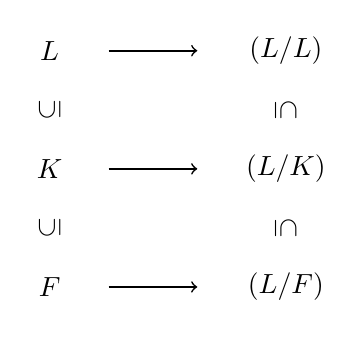
\begin{tikzpicture}[line width = 0.6, scale = 1.5]
\node (F2) at (0,2) {$L$}; 
\node (F1) at (0,1) {$K$}; 
\node (F) at (0,0) {$F$};
\foreach \i in {0.5,1.5} {\node[rotate =90] at (0,\i) {$\subseteq$};}

\node (H2) at (2,2) {$\Aut(L/L)$}; 
\node (H1) at (2,1) {$\Aut(L/K)$};
\node (H) at (2,0) {$\Aut(L/F)$};
\foreach \i in {0.5,1.5} {\node[rotate =-90] at (2,\i) {$\subseteq$};}

\foreach \i in {0,1,2} {\draw[->] (0.5,\i) -- (1.25,\i);}
\end{tikzpicture}
\end{center}

In the picture above we listed the group $\Aut(L/L)$. These are the automorphism of $L$ that fix all of $L$---there is only one such automorphism: the identity. Thus, $\Aut(L/L) = \{\text{id}\}$. 

Let's further explore these automorphism groups with some examples.

\begin{example}\label{exam.AutQAdjoinZeta5OverQ}
Let's try to compute $\Aut(\mathbb{Q}(\zeta_5/\mathbb{Q})$. First, we know that $x^4+x^3+x^2+x+1$ is the minimum polynomial for $\zeta_5$ over $\mathbb{Q}$, so by Theorem~\ref{thm.BasisExtensionField}  
\begin{itemize}
\item $\{1,\zeta_5,\zeta_5^2,\zeta_5^3\}$ is a basis for $\mathbb{Q}(\zeta_5)$ over $\mathbb{Q}$, and 
\item  $\mathbb{Q}(\zeta_5) = \{a+b\zeta_5+c\zeta_5^2+d\zeta_5^3\mid a,b,c,d\in \mathbb{Q}\}.$
\end{itemize}
Thus, every function $\phi\in \Aut(\mathbb{Q}(\zeta_5)/\mathbb{Q})$ can be expressed by a formula of the form \[\phi(a+b\zeta_5+c\zeta_5^2+d\zeta_5^3) = \text{ ??? }\]
Now, if $\phi\in \Aut(\mathbb{Q}(\zeta_5)/\mathbb{Q})$, then $\phi$ fixes $\mathbb{Q}$. By Theorem~\ref{thm.RingHomPlusLinearTrans}, $\phi$ is a $\mathbb{Q}$-linear transformation from $\mathbb{Q}(\zeta_5)$ to itself, and by a result from linear algebra, $\phi$ is completely determined by its values on a basis. That is, once we determine the values of $\phi(1)$, $\phi(\zeta_5)$, $\phi(\zeta_5^2)$, and $\phi(\zeta_5^3)$,  we will know a formula for $\phi$. In fact, this is easy to see directly: 
\begin{align*}
\phi(a+b\zeta_5+c\zeta_5^2+d\zeta_5^3) 
&= \phi(a)+\phi(b\zeta_5)+\phi(c\zeta_5^2)+\phi(d\zeta_5^3)\\
&= \phi(a)+\phi(b)\phi(\zeta_5)+\phi(c)\phi(\zeta_5^2)+\phi(d)\phi(\zeta_5^3)\\
&= a+b\phi(\zeta_5)+c\phi(\zeta_5^2)+d\phi(\zeta_5^3).
\end{align*}
In fact, we can take this further:
\begin{align*}
\phi(a+b\zeta_5+c\zeta_5^2+d\zeta_5^3)
&= a+b\phi(\zeta_5)+c\phi(\zeta_5^2)+d\phi(\zeta_5^3)\\
&= a+b\phi(\zeta_5)+c\phi(\zeta_5)^2+d\phi(\zeta_5)^3.
\end{align*}
So, to find a formula for $\phi$ we just need to determine the value for $\phi(\zeta_5)$; it can then be plugged into the above formula to find the value of $\phi$ on an arbitrary element of  $\mathbb{Q}(\zeta_5)$.

Now, since $\zeta_5$ is a root of $x^4+x^3+x^2+x+1$,  Theorem~\ref{thm.HomFixingFPermutesRootsOfPolysOverF} says that $\phi(\zeta_5)$ must be one of the roots of $x^4+x^3+x^2+x+1$, which are $\zeta_5$, $\zeta_5^2$, $\zeta_5^3$, and $\zeta_5^4$. The possibilities are named below. We will use repeatedly that $\zeta_5^5 = 1$;  if desired, we could also use $\zeta_5^4 = -\zeta_5^3-\zeta_5^2-\zeta_5-1$.
\begin{itemize}
\item $\phi_1$ sends $\zeta_5\mapsto \zeta_5$, which implies  $\phi_1(a+b\zeta_5+c\zeta_5^2+d\zeta_5^3) = a+b\zeta_5+c\zeta_5^2+d\zeta_5^3$;
\item $\phi_2$ sends $\zeta_5\mapsto \zeta_5^2$, which implies  $\phi_2(a+b\zeta_5+c\zeta_5^2+d\zeta_5^3) = a+b\zeta_5^2+c\zeta_5^4+d\zeta_5$;
\item $\phi_3$ sends $\zeta_5\mapsto \zeta_5^3$, which implies  $\phi_3(a+b\zeta_5+c\zeta_5^2+d\zeta_5^3) = a+b\zeta_5^3+c\zeta_5+d\zeta_5^4$;
\item $\phi_4$ sends $\zeta_5\mapsto \zeta_5^4$, which implies  $\phi_4(a+b\zeta_5+c\zeta_5^2+d\zeta_5^3) = a+b\zeta_5^4+c\zeta_5^3+d\zeta_5^2$.
\end{itemize}
Here's another way to organize the possibilities.
\begin{center}
\tabulinesep = 2mm
\begin{tabu} spread 1in {X[$c,m]|[2pt]X[$c,m]|X[$c,m]|X[$c,m]|X[$c,m]}
 & \phi_1 & \phi_2 & \phi_3 & \phi_4  \\ \tabucline[2pt]{-}
\zeta_5 \; \mapsto  & \zeta_5 & \zeta_5^2  & \zeta_5^3  & \zeta_5^4  
\end{tabu}
\end{center}
We now have to determine if each $\phi_i$ is in $\Aut(\mathbb{Q}(\zeta_5)/\mathbb{Q})$ or not. As $\phi_1$ is just the identity, $\phi_1 \in \Aut(\mathbb{Q}(\zeta_5)/\mathbb{Q})$. To check the other possibilities, we can use Fact~\ref{fact.SameMinPolyIsomorphic}. For example, Fact~\ref{fact.SameMinPolyIsomorphic} says that $\phi_2$ is an isomorphism from $\mathbb{Q}(\zeta_5)$ to $\mathbb{Q}(\zeta_5^2)$. Since $\mathbb{Q}(\zeta_5^2) =\mathbb{Q}(\zeta_5)$ (because $\zeta_5^2\in \mathbb{Q}(\zeta_5)$ and $\zeta_5\in \mathbb{Q}(\zeta_5^2)$), $\phi_2$ is indeed an automorphism of $\mathbb{Q}(\zeta_5)$, so $\phi_2 \in \Aut(\mathbb{Q}(\zeta_5)/\mathbb{Q})$. Similarly, $\phi_3,\phi_4 \in \Aut(\mathbb{Q}(\zeta_5)/\mathbb{Q})$. These are all possibilities, so 
\[\Aut(\mathbb{Q}(\zeta_5)/\mathbb{Q}) = \{\phi_1,\phi_2,\phi_3,\phi_4\} = \{\text{id},\phi_2,\phi_3,\phi_4\}.\]
\end{example}

We now know that $\Aut(\mathbb{Q}(\zeta_5)/\mathbb{Q})$ is a group of order $4$. What group is it? 

\begin{problem}
Let's determine what group $\Aut(\mathbb{Q}(\zeta_5)/\mathbb{Q})$ is isomorphic to. 
\begin{enumerate}
\item Which element of $\Aut(\mathbb{Q}(\zeta_5)/\mathbb{Q})$ is $(\phi_2)^2$ equal to? (Remember $(\phi_2)^2$ means $\phi_2\circ\phi_2$.)
\item Do the same for $(\phi_2)^3$ and $(\phi_2)^4$. Are either $(\phi_2)^3$ or $(\phi_2)^4$ equal to $\text{id}$? What is the order of $\phi_2$? (The order of $\phi_2$ will be the smallest positive $k$ such that $(\phi_2)^k = \text{id}$.)
\item What are the orders of $\phi_3$ and $\phi_4$?
\item Is $\Aut(\mathbb{Q}(\zeta_5)/\mathbb{Q})$ cyclic or not? Is $\Aut(\mathbb{Q}(\zeta_5)/\mathbb{Q})$ isomorphic to $\mathbb{Z}_4$ or $V_4$?
\end{enumerate}
\end{problem}

An important observation in Example~\ref{exam.AutQAdjoinZeta5OverQ} was that the possibilities for $\phi$ are determined simply by the possible values of $\phi(\zeta_5)$. This is true in general.

\begin{fact}\label{fact.AutDeterminedOnGenerator}
Let $F$ be a subfield of $E$. Suppose that $\alpha\in E$ is algebraic over $F$, and let $n$ be the degree of $\alpha$ over $F$. Then each $\phi\in \Aut({F}(\alpha)/F)$ is completely determined by the value $\phi(\alpha)$. Consequently,  $|\Aut({F}(\alpha)/F|\le n = [F(\alpha):F]$.
\end{fact}

\begin{problem}\label{prob.AutQAdjoinSqrt2OverQ}
Follow Example~\ref{exam.AutQAdjoinZeta5OverQ} to determine $\Aut(\mathbb{Q}(\sqrt{2})/\mathbb{Q})$.
What familiar group is  it isomorphic to?
\end{problem}

\begin{problem}\label{prob.AutQAdjoinCubeRoot2OverQ}
Let's determine $\Aut(\mathbb{Q}(\sqrt[3]{2})/\mathbb{Q})$.
\begin{enumerate}
\item First explain why  $\mathbb{Q}(\sqrt[3]{2})\neq \mathbb{Q}(\sqrt[3]{2}\zeta_3)$ and why $\mathbb{Q}(\sqrt[3]{2})\neq \mathbb{Q}(\sqrt[3]{2}\zeta_3^2)$.
\item Follow Example~\ref{exam.AutQAdjoinZeta5OverQ} to show that $\Aut(\mathbb{Q}(\sqrt[3]{2})/\mathbb{Q}) = \{\text{id}\}$.
\end{enumerate}
\end{problem}

What happens if we adjoin more than one element? Can we compute $\Aut(F(\alpha_1,\alpha_2)/F)$ in a similar way as to how we computed $\Aut(F(\alpha)/F)$? The answer is yes, and the starting point is the following analog of Fact~\ref{fact.AutDeterminedOnGenerator}.

\begin{fact}
Let $F$ be a subfield of $E$. Suppose that $\alpha_1,\ldots,\alpha_k\in E$ are algebraic over $F$. Then each $\phi\in \Aut({F}(\alpha_1,\ldots,\alpha_k)/F)$ is completely determined by the values of $\phi(\alpha_1),\ldots,\phi(\alpha_k)$. Consequently,  $|\Aut({F}(\alpha_1,\ldots,\alpha_k)/F|\le  [F(\alpha_1,\ldots,\alpha_k):F]$.
\end{fact}

\begin{problem}\label{prob.AutQAdjoinSqrt2AndiOverQ}
Let's determine $\Aut(\mathbb{Q}(\sqrt{2},i)/\mathbb{Q})$.
\begin{enumerate}
\item Let $\phi\in  \Aut(\mathbb{Q}(\sqrt{2},i)/\mathbb{Q})$. Explain why there are only two choice for $\phi(\sqrt{2})$ and only two choice for $\phi(i)$. What are they?
\item Combine the different possibilities for $\phi(\sqrt{2})$ and $\phi(i)$ to complete the table below.
\begin{center}
\tabulinesep = 2mm
\begin{tabu} spread 1in {X[$r,m]|[2pt]X[$c,m]|X[$c,m]|X[$c,m]|X[$c,m]}
 & \phi_1 & \phi_2 & \phi_3 & \phi_4  \\ \tabucline[2pt]{-}
\sqrt{2} \; \mapsto\;  & \sqrt{2} &  &  & \\  
i \; \mapsto \; & i &  &  &   
\end{tabu}
\end{center}
\item Follow Example~\ref{exam.AutQAdjoinZeta5OverQ} to determine $\Aut(\mathbb{Q}(\sqrt{2},i)/\mathbb{Q})$.
\item What familiar group is  $\Aut(\mathbb{Q}(\sqrt{2},i)/\mathbb{Q})$ isomorphic to?
\end{enumerate}
\end{problem}

\begin{problem}\label{prob.AutQAdjoinSqrt2AndiOverQLattices}
Set $L = \mathbb{Q}(\sqrt{2},i)$. In Problem~\ref{prob.AutQAdjoinSqrt2AndiOverQ} we determined $\Aut(L/\mathbb{Q})$. Let's connect the subfields of $L$ with subgroups of $\Aut(L/\mathbb{Q})$ using Theorem~\ref{thm.AutLOverKSubgroupAutLOverF}. 
\begin{enumerate}
\item Let $K_1 = \mathbb{Q}(\sqrt{2})$. Find $\Aut(L/K_1)$ by determining which of  $\phi_1, \phi_2,\phi_3,\phi_4$ are in $\Aut(L/K_1)$.
\item Repeat for $K_2 = \mathbb{Q}(i)$. Find $\Aut(L/K_2)$.
\item Repeat for $K_3 = \mathbb{Q}(i\sqrt{2})$. Find $\Aut(L/K_3)$.
\item Use Theorem~\ref{thm.AutLOverKSubgroupAutLOverF} to organize your findings by writing the appropriate elements in the boxes in the subgroup lattice of $\Aut(L/\mathbb{Q})$.
\begin{center}
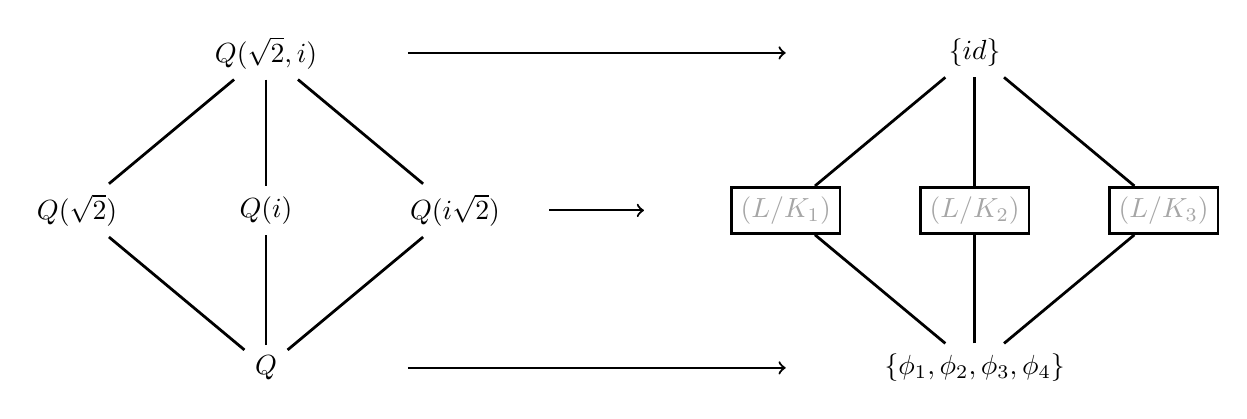
\begin{tikzpicture}[line width = 1, yscale = 1, xscale = 1.2]
\node (L) at (0,4) {$\mathbb{Q}(\sqrt{2},i)$}; 
\node (K1) at (-2,2) {$\mathbb{Q}(\sqrt{2})$}; 
\node (K2) at (0,2) {$\mathbb{Q}(i)$}; 
\node (K3) at (2,2) {$\mathbb{Q}(i\sqrt{2})$}; 
\node (F) at (0,0) {$\mathbb{Q}$};

\foreach \i in {1,2,3} {\draw (F) -- (K\i);}
\foreach \i in {1,2,3} {\draw (L) -- (K\i);}

\draw[line width = 0.8, ->] (1.5,4) -- (5.5,4);
\draw[line width = 0.8, ->] (3,2) -- (4,2);
\draw[line width = 0.8, ->] (1.5,0) -- (5.5,0);

\begin{scope}[shift = {(7.5,0)}]
\node (L) at (0,4) {$\{\text{id}\}$}; 
\node[draw] (K1) at (-2,2) {\textcolor{black!35}{$\Aut(L/K_1)$}}; 
\node[draw] (K2) at (0,2) {\textcolor{black!35}{$\Aut(L/K_2)$}};
\node[draw] (K3) at (2,2) {\textcolor{black!35}{$\Aut(L/K_3)$}};
\node (F) at (0,0) {$\{\phi_1, \phi_2,\phi_3,\phi_4\}$};

\foreach \i in {1,2,3} {\draw (F) -- (K\i);}
\foreach \i in {1,2,3} {\draw (L) -- (K\i);}
\end{scope}

\end{tikzpicture}
\end{center}
\end{enumerate}
\end{problem}

Problem~\ref{prob.AutQAdjoinSqrt2AndiOverQLattices} highlights quite well the tight connection between subfields of an extension field $L$ of $F$ and subgroups of $\Aut(L/F)$. So far, we've seen how each subfield $K$ gives rise to a subgroup $\Aut(L/K)$. The next theorem indicates how we might reverse this.

\begin{theorem}\label{thm.SubgroupAutLOverKYieldsSubfield}
Let $F$ be a subfield of $L$ and  $H$  a subgroup of $\Aut(L/F)$. Define \[\Fix_L(H) = \{k\in L \mid \text{$k$ is fixed by every $\phi \in H$}\}.\] Then $\Fix_L(H)$ is a subfield of $L$, and $F\subseteq \Fix_L(H) \subseteq L$.
\end{theorem}

The picture is as follows.
\begin{center}
\begin{tikzpicture}[line width = 0.6, scale = 1.5]
\node (F2) at (0,2) {$L$}; 
\node (F1) at (0,1) {$\Fix_L(H)$}; 
\node (F) at (0,0) {$F$};
\foreach \i in {0.5,1.5} {\node[rotate =90] at (0,\i) {$\subseteq$};}

\node (H2) at (2,2) {$\{\text{id}\}$}; 
\node (H1) at (2,1) {$H$};
\node (H) at (2,0) {$\Aut(L/F)$};
\foreach \i in {0.5,1.5} {\node[rotate =-90] at (2,\i) {$\subseteq$};}

\foreach \i in {1} {\draw[<-] (0.75,\i) -- (1.5,\i);}
\end{tikzpicture}
\end{center}


Taking a closer look at Problem~\ref{prob.AutQAdjoinSqrt2AndiOverQLattices}, we can see that the maps $K \mapsto \Aut(L/K)$ and $H \mapsto \Fix_L(H)$ are actually inverses of each other. For example, $\Fix_L(\Aut(L/K_1)) = K_1$, so the composition of the maps looks like $K_1 \mapsto \Aut(L/K_1) \mapsto \Fix_L(\Aut(L/K_1)) = K_1$. However, this is not true for all fields, and Problem~\ref{prob.AutQAdjoinCubeRoot2OverQ} gives an example. In the next chapter we'll study an important collection of fields (in fact, \emph{the} collection of fields) for which $K \mapsto \Aut(L/K)$ and $H \mapsto \Fix_L(H)$ are always inverses.


